% !TEX root = HDA_MDRL.tex

\section{Processing Pipeline}
\label{sec:processing_architecture}

We start off our analysis by preprocessing the collected signals within the MATLAB environment: we chose this framework because we find it is easier to operate with matrices. In this first step we import the data collected by sensors, which are given as \textit{'.dat'} files, then we select the signals from on-body sensors and discard the others, so we replace the missing values by means of interpolation and, at last, we store them as \textit{'.mat'} files.

Then, this time with python, we import the preprocessed data and make the dataset suitable for the classification task: this consists for example of segmenting data into windows, scaling and normalizing raw signals.

Finally, after the last step of preprocessing, we define and train a suitable learning model. This is respectively done for both the locomotion activity and gestures recognition, i.e. with two different sets of labels. The model, which is forced to learn also the null class together with the actual movements, is then compared to a different system where two stages are carried out; in that case, the first one has the purpose of detecting activity while the second one classifies the type of movement, if detected. Figure \ref{fig:pipeline} shows a schematic depiction of the comprehensive pipeline, which we are going to present in the following sections.

\begin{figure}[ht]
	\centering
	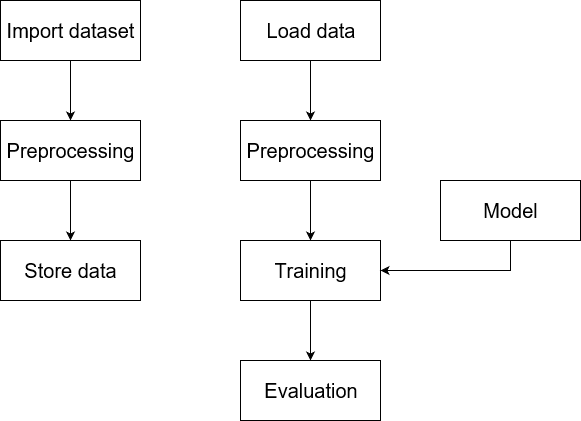
\includegraphics[scale=.4]{figure/block_diag}
	\title{Framework Pipeline}
	\caption{Framework Pipeline. On the left, the 3 block represent the process followed within the MATLAB framework; on the right instead, the pipeline for our python code.}
	\label{fig:pipeline}
\end{figure}

\section{Signals and Features}
\label{sec:model}

The OPPORTUNITY dataset, succinctly introduced in section \ref{sec:related_work}, has been collected from four subjects accomplishing different Activities of Daily Life (ADLs). As highlighted before, both the environment they moved in and the participants were meticulously monitored.
The process of acquisition consisted in 5 consecutive runs (named $ADL_1$ to $ADL_5$) that followed a predetermined script, plus a sixth run consisting of 20 repetitions of each activity present in the script (named \textit{Drill} run). Each vector of samples corresponding to a single time-step is assigned with a distinct set of labels: in the following we'll refer to Task A when we consider high-level modes of locomotion (\textit{Standing, Walking, Sitting, Lying}), while we'll refer to Task B for more specific arm gestures (17 in total). To these tasks we need of course to add the \textit{Null Class} that we mentioned earlier in this paper: specifically, this label represents the state in which the participant does nothing (or something that is not considered among the listed classes). 

The wireless sensors worn by the subjects (IMU - Inertial Measurement Unit) provide acceleration among the three-axes, rate of turn, magnetic field and orientation information; in addition, 12 accelerometers were placed on the subjects' parts of the body sensible to movements (arms, back, hips and feet). Figure \ref{fig:sensors} shows how these sensors were placed on the body. All these devices acquired together a total of 145 distinct channels but, for the purposes of our work, we base the analysis only on on-body sensor signals, considering just 113 channels.

\begin{figure}[ht]
	\centering
	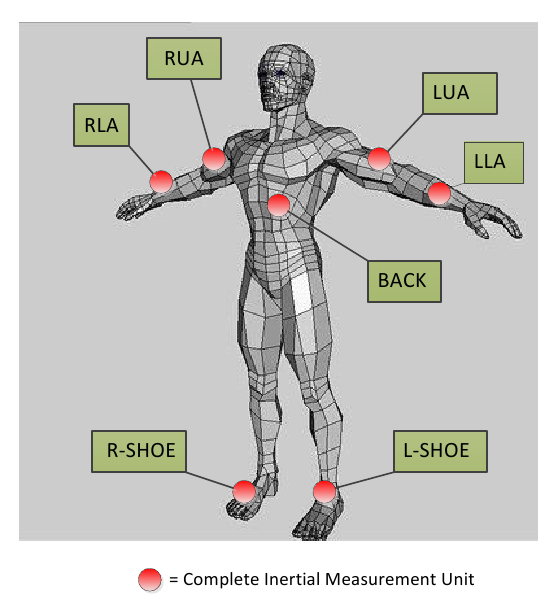
\includegraphics[scale=.29]{figure/Fig1Cl} \hfil
	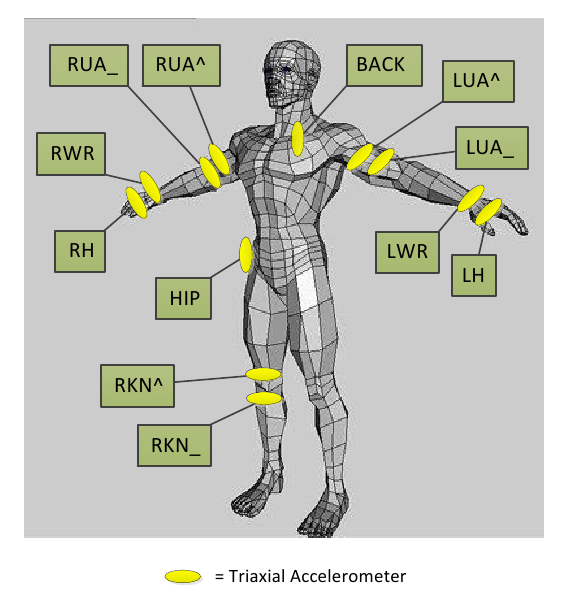
\includegraphics[scale=.29]{figure/Fig1Cr}
	\title{Sensor Locations.}
	\caption{Sensor Locations. The two images show the locations of on-body sensors for the measurements of the OPPORTUNITY dataset. The first image shows complete \textit{Inertial Measurement Units}, while the second shows \textit{Triaxial Accelerometers}.}
	\label{fig:sensors}
\end{figure}

Since sensors were wireless, the collected signals could present some missing data, which are indicated with NaN values. These manifest mostly as bursts and thus, in the preprocessing phase, we performed spline interpolation with a cubic polynomial; however, this type of interpolation ends up meaningless if more than the 30\% of data is missing. For this reason we had to discard all the three columns corresponding to one of the physical devices: this led us to work with 110 channels. Since we noticed that the head and tail of the measurement sessions correspond to a transient where most of the sensors are turned-off, we decided to discard them. In this way we ensure that the interpolation phase provides consistent results; the subsequent step consists in normalizing each column with respect to mean and variance. After that, in order to instruct the framework on one subject, we stack sessions from $ADL_1$ to $ADL_3$ and \textit{Drill} as a first step to create our training set; then, we assemble also $ADL_4$ and $ADL_5$ to build the test set. 

To conclude the preprocessing phase, finally we decided to follow the same procedure as in several works we cited earlier: we apply in fact the \textit{sliding window} technique on the datasets, obtaining a tensor of windows constituted of 15 samples (500 ms), using a stride of length 5. In our case, we decided to assign to each window the most frequent label: this doesn't constitute a problem per se, even when changing the size of the sliding window, as long as it is kept short enough for being representative of a movement.

We found in fact that the choice of window size and stride is fundamental in order to obtain good results: we observed that a window too short can't represent a single gesture with fair precision and, on the contrary, if the window is too large we could include two distinct movements (or modes of locomotion), leading to non significant labelling. The choice of the size of the displacement separating two consecutive windows can guarantee a good trade-off between windows diversity and dataset population.

In the first phase of our project we also tried to create a reduced dataset of features: since each accelerometer returns the acceleration value in the direction of all the three axes, we tried to substitute these three values with a unique value representing the \textit{mean acceleration} measured by the sensors. In our first experiments, however, this led to poor results: with respect to the simulations where all features were fed to the model, the configuration using the reduced dataset was affected by almost a 5\% loss in terms of accuracy. 

\section{Learning Framework}
\label{sec:learning_framework}

\begin{table}[]
	\begin{tabular}{lccc}
		\textbf{Model name}        & \textbf{Convolutional} & \textbf{Recurrent} & \textbf{Fully connected} \\
		Conv              & 3             & 0         & 2			   \\
		Conv1DRecurrent   & 1             & 2         & 2               \\
		Conv2DRecurrent   & 1             & 2         & 2               \\
		ConvDeepRecurrent & 3             & 2         & 2
	\end{tabular}
	\caption{Model architectures. The number of different layers stacked in each models is here reported. 'Conv' stands for 'Convolutional'.}
	\label{tab:models}
\end{table}

One of the main problems in Human Activity Recognition is handling \text{inactivity}. Since we segmented our signals with a sliding window approach, we resulted in having portions of signals associated to a unique label: this label is null when the subject is idle during most of the time window. Thinking of a real-time recognition system, we can implement two different strategies to deal with this class, which are reported below in \ref{sub:oneshot} and \ref{sub:twosteps}.

\subsection{One Shot Classification}
\label{sub:oneshot}

This classification technique uses just one model to predict whether there is activity and of which type: e.g. an n-class classification in this case becomes a (n+1)-class classification, because even the \textit{Null Class} is considered as an activity. We think that this process fits particularly simpler classification tasks, because the number of operations is constant during each time window: this means that even when the subject is idle, the system has to perform the same operations, with the same energy consumption.

\subsection{Two Steps Classification}
\label{sub:twosteps}

As an alternative, the process can be split into two steps: one to detect activity and one to recognize it when present. In practice the first step receives signal windows and decides if the subject is active or inactive, performing thus a binary classification; then, only if it’s labelled as active, the signal is passed to a second model which tries to recognize the activity. This approach could be particularly appealing in real-time systems, especially if the detection phase has a low number of operations: considering that in daily life recordings one is mostly idle, this leads to a decreased energy consumption. A major drawback though is that the final accuracy of the model is affected by the errors made by both the models: even having a good classification model would be inefficient if it were passed, erroneously, mostly inactivity signals. This suggests that there’s a trade-off in activity detection task between accuracy and energy consumption. Luckily enough this phase could also be effective exploiting non deep learning techniques, which anyway aren't explored in our work.\\

To test our pipelines we implemented 4 different models, named \textit{Convolutional, Convolutional1DRecurrent, Convolutional2DRecurrent} and \textit{ConvolutionalDeepRecurrent}. The four of them, reported by increasing complexity, use some convolutional layers and, exception made for the first one, a couple of recurrent layers with LSTM units. A superficial comparison between their architectures is given in table \ref{tab:models}, where we specified the number of layers per type. 
These models are tested and compared on different tasks so, to use them properly, the last fully connected layer of each one has the number of units required by the specific task, which depends on the pipeline selected. The final choice of all the hyper-parameters (size of convolutional kernels, size of pooling windows, number of cells per LSTM layers, etc) has been done via fine-tuning and consecutive trials: other options could have been grid search or Bayesian learning, however we didn't investigate them in this paper.

Among many experiments, we also tried to add an SVM layer in order to boost our performances: however, considering that we obtained just a slight improvement, the additional computational effort needed to evaluate the features wasn't worth it. 
